    \documentclass[12pt]{article}
\usepackage[labelfont=bf]{caption}
\captionsetup[table]{labelsep=space, 
         justification=raggedright, singlelinecheck=off}
\usepackage[margin=1in]{geometry} 
\usepackage{amsmath,amsthm,amssymb}
\usepackage{hyperref}
\usepackage{graphicx}
\usepackage{xcolor}
\usepackage[many]{tcolorbox}
\tcbuselibrary{listings}
\usepackage{listings}
\usepackage{float}
\definecolor{lg}{HTML}{f0f0f0}

\newtcblisting{pycode}{
    colback=lg,
    boxrule=0pt,
    arc=0pt,
    outer arc=0pt,
    top=0pt,
    bottom=0pt,
    colframe=white,
    listing only,
    left=15.5pt,
    enhanced,
    listing options={
        basicstyle=\small\ttfamily,
        keywordstyle=\color{blue},
        language=Python,
        showstringspaces=false,
        tabsize=2,
        numbers=left,
        breaklines=true
    },
    overlay={
        \fill[gray!30]
        ([xshift=-3pt]frame.south west)
        rectangle
        ([xshift=11.5pt]frame.north west);
    }
}

\lstset{
    language=Python,
    basicstyle=\small\ttfamily,
}

 
\begin{document}
 
\title{Pong Report}
\author{Cristian Abrante, Alejandro Esquivias\\

ELEC-E8125 - Reinforcement Learning}

\maketitle
\section{Introduction}
The purpose of this project is to implement a Reinforcement Learning agent that can play Wimblepong. In the first section, we will review some external sources that discuss this problem. In the second second section we will explain our agent's architecture. The third section will focus on the training methodology. Finally, in the fourth section we will discuss our results and we will conclude this project.

\section{Review of external sources}

In this section, we are going to explain the reinforcement learning algorithm implemented in order to train the agent. First of all, we explored the paper \textit{"Playing Atari with deep Reinforcement Learning"} \cite{mnih2013playing}, which was a good example for understanding which was the previous works done when trying to solve this type of problems using reinforcement learning techniques. But after that, we focused on the work presented by OpenAI, one of the most prominent artificial intelligence research laboratories nowadays, where they described a method that combines three desirable features: easy to implement, efficient in sampling and easy to hypertune. This method is Proximal Policy Optimization (PPO) \cite{schulman2017proximal}. \\

PPO is an on-policy method that does not use experience replay in order to learn from a batch of past transitions. On the contrary, it updated the weights of the policy network based on the results obtained in the current execution of the episode. This caused that this method is sample efficient, for example in comparison with Deep Q-Learning \cite{gu2016continuous}, which used a batch of experience replay which can be significantly big.\\

To explain PPO, we have to start by explaining the loss function that policy gradient methods have:

\begin{equation}
    L^{PG}(\theta) = E_t[log\pi_{\theta}(a_t|s_t)A_t]
\end{equation}

As we can see, the loss function is the expectation of the log function of the probability using the current policy ($\theta$) of selecting the action $a_t$, having the state $s_t$. This is multiplied by the advantage term ($A_t$), which is the proportional importance that the past action had in the outcome. The problem that this method have is that if we run gradient descent on a single batch of collected experience, the update of the weights could be really far from each other and can lie to extremely worst results when updating the policy. \\

This loss function is updated using Trust Region Policy Optimization (TRPO) \cite{schulman2015trust}, which is the basis in which PPO relies, and which updated the loss function using the following equation:

\begin{equation}
    L^{TRPO}(\theta) = E_t[\frac{log\pi_{\theta}(a_t|s_t)}{log\pi_{\theta_{old}}(a_t|s_t)}A_t]
    \label{ppo-loss}
\end{equation}

The fraction between the log probabilities works as a sort of normalization constraint, to prevent the policy to diverge in a significant way between iterations. Starting from this basis, PPO adds a clipping constraint for making sure that this true area is not overpassed. The result of the loss function is this formula:

\begin{equation}
    L^{PPO}(\theta) = E_t[min\{\frac{log\pi_{\theta}(a_t|s_t)}{log\pi_{\theta_{old}}(a_t|s_t)}A_t, clip(\frac{log\pi_{\theta}(a_t|s_t)}{log\pi_{\theta_{old}}(a_t|s_t)}, 1-\epsilon, 1+\epsilon)A_t\}]
\end{equation}

This function uses the minimum of two elements, on the one hand is the normal TRPO loss, which pushes the network to have intensive updates, and on the other hand it is the clipped version that restricts the function into a certain range defined by a constant $\epsilon$.

\section{Design of the agent architecture}.

After having explained the reinforcement learning algorithm that we used to solve our problem, we are going to explain how we designed the agent and the neural network that was used to learn the optimal policy.\\

But first, we are going to describe the different auxiliary methods that we used:

\begin{itemize}
  \item \texttt{preprocess\_image}: Method used to preprocess the image. We take the pixels two by two to perform dimensionality reduction. Then, we compare the reduced image with the background. If they are not equal to the background that pixel is set to $1$ and otherwise is set to $0$. This is done to highlight the important elements.
  \item \texttt{discount\_rewards}: This function returns the discounted rewards given gamma parameter ($\gamma$).
  \item \texttt{substract\_observations}: This function is used to substract the pixels from two images. If we have only received one observation (start of the episode) then the returned image is the preprocessed image (returned with the \texttt{preprocess\_image} method we described earlier).
\end{itemize}

After that, we are going to describe the \texttt{Agent} class. The main function of the agent is to return the desired action given a certain observation (pixel image), and to update the policy using PPO algorithm and the loss function described in the last section. \\

The main methods that it contains are:

\begin{itemize}
    \item \texttt{\_\_init\_\_}: In the initialization method we define the hyperparamaters and some class parameters, such as observations vector, actions vector, actions probability vector and the rewards vector. Also, it is important to mention that the policy that the agent is going to follow has to be passed to this initialization.
    
    \item \texttt{get\_action}: Thanks to this method our agent can choose an action from an observation. We return the action and the action probability.
    
    \item \texttt{update\_policy}: In this function is where we update the policy using the PPO algorithm and the loss function described by equation \ref{ppo-loss}.
\end{itemize}

Finally, we are going to explain the \texttt{Policy} class, which is going to be the neural network that it is going to learn the policy. The methods of this class are the common ones when extending a Pytorch module:

\begin{itemize}
    \item \texttt{\_\_init\_\_}: In the initialization method we define the neural network's architecture. We are going to explain this architecture in depth later on.
    \item \texttt{forward}: This is the forward propagation of the observation using the convolutional and linear layers. Notice that before forwarding through the linear layers we need to reshape thanks to the view function without knowing the number of columns.
\end{itemize}

After defining the methods, we are going to explain the selected network architecture. For doing that, we are considering that the input is the reduced 100x100 image of the pong environment. This is the diagram of the network: \\

\begin{figure}[h]
    \centering
    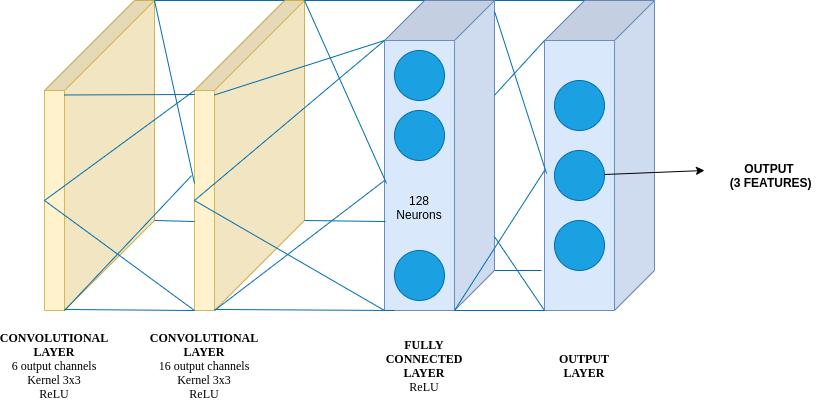
\includegraphics[scale=0.3]{Untitled Diagram (1).png}
    \label{fig:my_label}
\end{figure}

We are going to explain separately the parts of the architecture:

\begin{itemize}
    \item \textbf{Convolutional layer}: First convolutional layer of 6 channel output, and a kernel of 3x3. this layer is used as the first input of the network and we decided to follow a classic approach when processing images, so this is why we fixed those values and used a ReLU activation function after it.
    \item \textbf{Second convolutional layer}: The second convolutional layer accepted the 6 channels of the previous one, and produced 16 output channels, in order to detect more complex features. As in the previous case, we used ReLU activation function. 
    \item \textbf{First linear layer}: Linear layer accepted a flattened version of the neural network and then used 128 internal neurons to produce the output. One important improvement that could be done here is to increase the number of internal neurons in order to increase the capacity of detection.
    \item \textbf{Output layer}: accepting the 128 input of the previous layer, the final layer produces the logits with 3 channels. Those three logits are the probabilities that are going to be taking from sampling an action from a categorical distribution.
\end{itemize}

\section{Training methodology}

We created a custom main.py file to train the agent against \textit{Simple AI}. At first it was not performing properly and we were getting NaN values and Runtime errors. This was due to the learning rate being too high. After reducing the learning rate we let it train for 500 episodes and the results can be seen in the next section. We tried different learning rates over 500 episodes and picked the one with the highest win-rate. The second problem we faced was that we did not fully respect the interface requirements, since we were at first doing the preprocessing before passing the observation to the get\_action method. Nonetheless, this should not have affected the \texttt{.mdl} file where all the model weights were saved.

\section{Evaluation of results}
After training, as mentioned in the previous section, we obtained the following results.

\begin{figure}[H]
    \centering
    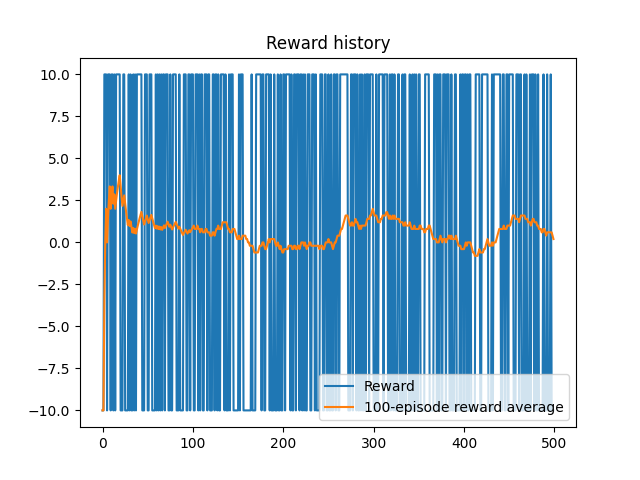
\includegraphics[scale=0.7]{reward2.png}
    \caption{Graph displaying the rewards, with the orange line representing an average over 100 episodes.}
   
\end{figure}

\begin{figure}[H]
    \centering
    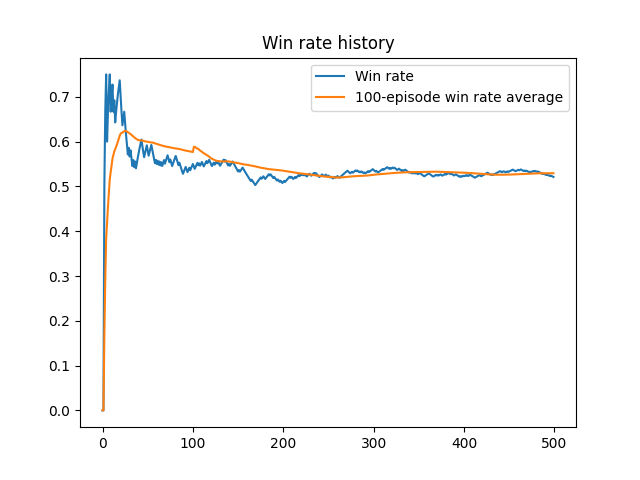
\includegraphics[scale=0.7]{win rate-hist.png}
    \caption{Graph displaying the win-rate and win-rate average over 100 episodes.}
   
\end{figure}
As we can see, the rewards remain quite stable after iteration number 25. This could indicate that more time is needed to train the model, with a more complex neural network to process better the difference in observation input. The win-rate after 500 episodes is approximately 0.52, meaning the agent wins 52\% of the time. Due to the high dimensionality of the problem, more training time is required.
\section{Conclusions}

In conclusion, our agent performed reasonably well for the little amount of time we trained it (0.52 win-rate after 500 episodes), but would most likely not be competitive against a well-trained DQN or against a human player.\\

To improve the performance of the agent we could develop a more complex neural network, especially using more hidden layers, more neurons, and a better selection of convolutional layers. Apart from that, more advanced techniques such as MaxPooling could be applied to improve the results of the convolutional layers. Secondly, the hyperparameter tuning was not done in a correct way, we should develop a correct hyperparameter grid test in order to select the different parameters: optimizer of the network, learning rate of it, and also architectural parameters such as the number of hidden neurons or the activation functions used in them.

\bibliographystyle{ieeetr}
\bibliography{template}  % Modify template with your bibliography name
\end{document}
